\usepackage[ManyBibs,LabelsAligned,NoDate]{currvita} % currvita style
\usepackage[export]{adjustbox}

% Symbols and SVGs via TikZ
\usepackage{fontawesome5}
\usepackage{tikz}
\usetikzlibrary{svg.path}

\usepackage{scalerel}

\tikzset{
	orcid/.pic={
		\fill svg[scale=.001ex] {%
			M1309.33 948.955c-25.234 11.776-49.078 19.676-71.68 23.406-22.528 3.876-58.66 5.706-108.69 5.706h-129.902v-540.598h133.194c51.932 0 92.306 3.584 121.124 10.678s52.81 16.018 72.046 26.99c19.236 10.898 36.864 24.284 52.882 40.302 51.274 52.078 76.946 117.76 76.946 197.194 0 78.044-26.332 141.75-79.068 191.050-19.456 18.286-41.838 33.426-66.852 45.276zM1024 1609.143c-484.79 0-877.714-392.996-877.714-877.714s392.924-877.714 877.714-877.714 877.714 392.996 877.714 877.714-392.924 877.714-877.714 877.714zM732.598 343.845h-104.010v726.82h104.010v-726.82zM680.522 1146.587c-39.424 0-71.534 31.89-71.534 71.534 0 39.35 32.036 71.46 71.534 71.46 39.57 0 71.606-32.036 71.606-71.46-0.074-39.716-32.036-71.534-71.606-71.534zM1534.83 567.589c-18.724-44.398-45.422-83.456-80.164-117.102-35.328-34.816-76.434-60.854-123.318-78.556-27.428-10.678-52.516-17.92-75.41-21.65-22.966-3.584-66.634-5.34-131.218-5.34h-229.888v725.724h245.028c98.962 0 177.078-14.702 234.716-44.398 57.564-29.622 103.278-73.362 137.29-130.852 34.012-57.564 51.054-120.394 51.054-188.27 0.074-48.714-9.436-95.232-28.086-139.556z};
	}
}

\newcommand\orcid{\mbox{\scalerel*{
			
\begin{tikzpicture}[transform shape]
				\pic{orcid};
			\end{tikzpicture}
		}{\textnormal |}}}

\tikzset{
	publons/.pic={
		\fill svg[scale=.001ex] {%
			M1582.022 1339.517c-14.724 35.914-35.818 68.878-59.392 99.548-56.188 70.956-130.392 131.16-218.872 155.414-132.966 36.768-280.35 1.894-388.798-81.568-23.304-17.664-43.988-38.348-63.136-60.342-9.172 47.47-12.018 96.022-22.77 143.126-5.508 5.918-10.84 14.774-20.32 13.282-23.582-0.454-45.48-10.386-66.94-19.148-92.452-40.2-184.59-81.028-277-121.176-9.758-4.652-21.958-7.050-28.19-16.764-2.034-13.012-1.894-26.514-0.138-39.57 5.602-12.822 19.558-18.688 30.902-25.6 29.806-16.758 61.922-30.53 88.072-53.072 23.486-19.332 35.906-49.050 38.034-78.95 0.944-9.896 1.266-19.83 1.31-29.806-0.088-362.87 0.052-725.782-0.088-1088.65-2.348-45.846 0.636-92.094-6.73-137.574-3.796-21.408-16.076-45.348-39.476-49.59-35.050-2.706-70.414 1.31-105.414-1.806-9.354-0.358-12.646-10.526-12.062-18.38 0.088-20.868-0.586-41.78 0.358-62.69-0.044-5.734 6.188-8.448 9.398-12.376 65.398 1.712 130.758 6.458 196.154 7.226 125.016 2.436 250.126 0.226 374.922-7.314 9.802-0.044 25.248-0.182 27.414 12.236 1.946 22.316 1.674 44.938 0.182 67.21-0.182 9.896-10.254 14.592-18.834 14.592-27.012 1.398-54.016 0.176-81.028 0.454-15.712 0.41-32.79-1.894-47.104 6.1-14.27 8.668-19.244 26.016-23.084 41.238-11.382 57-7.182 115.492-9.304 173.216-1.404 128.314-3.342 256.636-3.796 384.994 53.116-23.94 110.796-36.404 168.652-41.508 100.498-9.662 204.062 10.21 292.726 58.85 111.696 59.984 197.428 162.334 245.84 278.682 38.348 91.194 55.238 190.734 53.526 289.426-0.33 68-8.462 137.15-35.020 200.294zM1337.674 809.627c-19.916-70.964-60.248-141.056-127.056-176.83-56.364-31.386-124.072-27.546-185.27-15.404-47.514 9.398-90.646 33.828-127.012 65.222-31.114 30.442-42.686 75.564-42.094 117.972 0.592 184.73-0.856 369.554 0.724 554.24 41.684 58.448 109.436 96.248 180.122 105.962 67.116 9.846 138.116-12.244 186.448-60.072 65.492-63.818 97.828-153.292 116.802-240.874 22.674-115.082 29.002-236.17-2.662-350.216z};
	}
}

\newcommand\publons{\mbox{\scalerel*{
			
\begin{tikzpicture}[transform shape]
				\pic{publons};
			\end{tikzpicture}\phantom{.}
		}{\textnormal p}}}

\tikzset{
	researchgate/.pic={
		\fill svg[scale=.001ex] {%
			M1194.642 23.429c-93.996 102.282-219.786 266.57-324.426 452.286
			172.852 40.426 300.852 202.716 300.852 364.858 0 239.002-185.636
			349.93-428.998 349.93-125.784 0-226.144-6.356-319.854-6.356-85.504
			0-170.934 0-224.146 2.070v-61.93l80.998-14.856c55.712-10.716
			87.428-36.148
			87.428-168.572v-840.646c0-132.36-31.714-157.93-87.428-168.5l-80.998-15.14v-61.718c57.57
			2.070 157.856 6.29 258.216 6.29 96 0 219.786-4.22
			273.144-6.29v61.718l-111.002 15.14c-57.564 8.36-87.574 36.14-87.574
			168.5v356.286c51.214-4.286 96-4.286 164.432-4.286 130.144-232.5
			253.922-407.566 324.214-488.572 64.138-76.924 162.216-125.93
			285.996-125.93 36.22 0 74.584 6.364 98.004 17.144v55.362c-76.786
			0-153.57 53.424-208.86 113.21zM684.5 548.287c-72.572 0-104.426
			1.93-153.644 6.568v535.362c49.218 4.286 115.214 4.286 172.858 4.286
			179.354 0 285.93-94.004 285.93-264.572
			0-168.572-115.142-281.644-305.144-281.644zM1335.86 1086.859c-2.144
			11.212-4.074 24.284-5.786 39.358-1.784 15.214-2.934 33.068-3.642
			54.14-0.716 20.926-1.002 46.496-1.002 75.784 0 29.432 0.286 54.646
			1.002 75.644 0.71 21.072 1.858 39.146 3.642 54.214 1.712 15.002
			3.642 28.146 5.786 39.358 2.070 11.286 4.784 22.002 8.288 32.498
			18.352 55.5 48.428 97.214 90.5 125.22 41.998 28 93.498 42.064
			154.638 42.064 31.43 0 59.934-3.642 85.218-11.066 25-7.358
			47.426-17.504 67.21-30.5 19.5-12.858 36.36-28 50.286-45.144
			14.284-17.21 25.782-35.57 34.786-55.288 3.496-6.282
			2.502-11.286-3.072-14.782l-77.642-31.926c-6.576-3.504-11.212-1.718-14.862
			5.216-17.422 32.286-32.286 53.496-56.708 68.922-24.714 15.36-47.572
			22.646-85.218 22.646-40.93
			0-59.216-8.14-84.854-26.5-25.432-18-44.076-40.646-55.076-75.14-2.208-6.218-4.214-13.934-6.568-23.004-1.93-9.216-3.504-20.502-4.498-33.712-1.002-13.216-1.93-29.572-2.786-48.86-0.57-19.288-0.856-42.716-0.856-69.858
			0-27.282 0.286-50.71 0.856-69.998 0.856-19.214 1.784-35.57
			2.786-48.786 0.994-13.356 2.568-24.568 4.498-33.858 2.356-8.93
			4.36-16.64 6.568-22.93 11-34.356 26.72-53.138 49.862-68.214
			22.858-15.286 49.138-26.288 90.068-26.288 36.36 0 69.646 10.358
			91.356 26.148 21.504 15.784 39.358 36.638 47.36 65.142 3.504 12.002
			8.002 26.932 11.074 45.216 2.786 18.286 2.786 37.64 2.786 64.352 0
			4.22-2.362 6.364-6.29 6.364h-124.358c-7 0-10.43 3.424-10.43
			10.422v71.286c0 7.072 3.43 10.504 10.43 10.504h228.214c7.146 0
			10.504-3.43 10.504-10.504v-60.928c0-32.286
			0-62.216-3.358-89.93-3.218-27.714-7.57-51.712-13.070-69.208-17.43-54.792-45.070-93.792-87.428-122.858-42.504-29.286-97.288-45.070-156.79-45.070-61.14
			0-112.64 14.066-154.638 41.998-42.072 28.284-72.148 69.786-90.5
			125.286-3.504 10.496-6.218 21.284-8.288 32.57z};
	}
}

\newcommand\researchgate{\mbox{\scalerel*{
			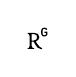
\begin{tikzpicture}[transform shape]
				\pic{researchgate};
			\end{tikzpicture}
		}{\textnormal R\textsuperscript{G}}}}

\tikzset{
	googlescholar/.pic={
		\fill svg[scale=.001ex] {%
			M1624.144 1414.115v124.49l90.354 70.538h-977.782l-590.432-513.25h391.57c-0.71-9.714-1.002-18.498-1.002-28.46 0-95.29 33.002-174.11 99.072-237.078 66.070-63.072 147.434-94.39 243.778-94.39 22.506 0 44.574 1.682 66.004 4.682-13.29-29.718-19.998-57.248-19.998-82.936 0-45.144 20.568-93.396 61.564-144.648-179.354-12.208-311.136-44.492-395.14-96.746-48.142-29.71-86.858-67.218-116.070-112.142-29.214-45.254-43.784-93.784-43.784-146.11 0-44.106 9.428-83.822 28.43-119.142s43.784-64.322 74.57-86.784c30.712-22.71 66.144-41.604 106.144-57 39.928-15.286 79.572-26.142 119.136-32.286 39.438-6.136 78.65-9.136 117.512-9.136 61.572 0 123.216 7.928 185.358 23.712 61.996 15.93 120.138 39.504 174.496 70.824 54.214 31.108 98.356 73.538 132.214 126.712 33.784 53.394 50.718 113.394 50.718 179.822 0 50.358-10.284 96.176-30.858 137.786-20.428 41.472-45.43 75.616-75.212 102.144-29.718 26.572-59.428 50.996-89.212 72.996-29.718 22.148-54.858 44.574-75.286 67.716-20.502 23.070-30.786 45.962-30.786 68.498 0 22.498 7.928 44.214 23.844 65.214 15.792 21.072 35.080 41.362 57.644 60.826 22.572 19.426 45.144 40.996 67.642 64.608 22.498 23.53 41.786 54.068 57.644 91.466 15.93 37.39 23.786 79.748 23.786 126.888 0 61.498-11.644 111.82-34.502 152.29-2.714 4.674-5.566 8.244-8.572 13.816l260.148 213.358v-78.256c-33.8-4.25-30.282-24.438-30.282-48.618v-588.192c0-27.238 22.286-49.526 49.526-49.526h18.234c27.238 0 49.526 22.286 49.526 49.526v588.192c0 24.122 3.554 44.288-29.996 48.596zM1133.356 397.071c5.216-3.43 16.932-12.712 35.284-27.604 18.512-14.826 31.072-26.038 37.786-33.894 6.576-7.606 16.362-19.040 29.148-34.502 12.858-15.426 21.57-28.818 26.142-39.928 4.572-11.322 9.216-24.964 13.926-40.894 4.506-15.748 6.788-31.89 6.788-48.282 0-77.934-30.004-135.68-89.856-173.070-60-37.398-131.504-56.108-214.572-56.108-41.998 0-83.214 4.996-123.714 14.606-40.426 9.676-79.14 24.394-116.070 43.894-36.93 19.464-66.64 46.644-89.146 81.356-22.572 34.926-33.858 75.038-33.858 119.998 0 47.178 12.786 88.182 38.502 122.998 25.57 34.86 59.144 61.22 100.718 79.156 41.428 18.038 83.426 30.822 125.996 38.392 42.57 7.782 85.928 11.68 130.004 11.68 20.428 0 36.278-1.148 47.564-3.182 2.078-1.002 13.86-9.464 35.358-25.432 21.504-15.828 34.86-25.578 40.002-29.184zM1118.004 856.855c-33.858-40.5-81.072-60.746-141.502-60.746-54.214 0-101.932 21.782-142.928 65.426-41.142 43.534-70.502 92.928-88.43 148.254-18 55.354-26.998 109.642-26.998 162.962 0 62.602 16.436 115.894 49.284 159.89 32.856 44.112 79.996 66.216 141.43 66.216 54.286 0 102.282-23.032 143.712-69.288 41.574-46.102 71.358-97.888 89.22-155.282 17.928-57.322 26.85-112.136 26.85-164.498 0-61.47-16.926-112.502-50.636-152.934z};
	}
}

\newcommand\googlescholar{\mbox{
		
\begin{tikzpicture}[transform shape,baseline=.16\baselineskip]
			\pic{googlescholar};
		\end{tikzpicture}
}}

\tikzset{
	envelope/.pic={
		\fill svg[scale=.001ex] {%
			M502.3 190.8c3.9-3.1 9.7-.2 9.7 4.7V400c0 26.5-21.5 48-48 48H48c-26.5 0-48-21.5-48-48V195.6c0-5 5.7-7.8 9.7-4.7 22.4 17.4 52.1 39.5 154.1 113.6 21.1 15.4 56.7 47.8 92.2 47.6 35.7.3 72-32.8 92.3-47.6 102-74.1 131.6-96.3 154-113.7zM256 320c23.2.4 56.6-29.2 73.4-41.4 132.7-96.3 142.8-104.7 173.4-128.7 5.8-4.5 9.2-11.5 9.2-18.9v-19c0-26.5-21.5-48-48-48H48C21.5 64 0 85.5 0 112v19c0 7.4 3.4 14.3 9.2 18.9 30.6 23.9 40.7 32.4 173.4 128.7 16.8 12.2 50.2 41.8 73.4 41.4z};
	}
}

\newcommand\envelope{\mbox{\scalerel*{
			\begin{tikzpicture}[transform shape, rotate=180]
				\pic{envelope};
			\end{tikzpicture}
		}{\textnormal l}}}

\newcommand{\raisedrule}[2][0em]{\leaders\hbox{\rule[#1]{1pt}{#2}}\hfill}
\newcommand{\heading}[1]{\vspace*{1em}\noindent\marginpar{\textcolor{black}{ \rule[.33\baselineskip]{\marginparwidth}{.66pt}}}{\color{black}\Large\scshape #1}\hspace{\marginparsep}\textcolor{black}{\raisedrule[.33\baselineskip]{.66pt}\vspace*{1em}}}
% Margin text style
\newcommand{\info}[1]{\marginpar{\raggedleft{\small #1}\vspace{-4em}}}
% Date box width
% CV entry
\newcommand\entry[3]{\noindent\hangafter=0\info{#1}{\color{black}#2}\hfill{\small #3} % Define a command for each new block - change spacing and font sizes here: #1 is the left margin, #2 is the italic date field and #3 is the position/employer/location field
	\nopagebreak[4]\par\vspace{0.5em}} % Add some white space after each new entry
% Entry description (goes well with \info)
\newcommand{\desc}[1]{\hangafter=0\noindent{#1}\par\vspace{1em}}
% Make it easier to handle linked email addresses
%\newcommand\reference[1]{\info{Reference}{\small#1}}
\newcommand{\email}[1]{\href{mailto:#1}{#1}}
\newcommand{\link}[1]{\href{#1}{#1}}

% Publications
\addbibresource[label=articles]{cv/articles.bib}
\addbibresource[label=talks]{cv/talks.bib}